\chapter{Methods}
\label{cha:methods}
This chapter contains the methods used for extending the existing hash based digital signature systems in this work.

\section{T5 Hashing}
Dodis et al.~\cite{T5_paper} propose a method called $T5$ for hashing five inputs with three hash compression calls. The $5n$-to-$n$ compression function $T5$ (with $n$ being the hash digest length) is constructed out of $2n$-to-$n$ compression functions $h_1, h_2, h_3$:

\begin{equation}
\label{eq:t5_basic}
T_5(m_1, m_2, m_3, m_4, m_5) = h_3(h_1(m_1,m_2) \oplus m_5, h_2(m_3,m_4) \oplus m_5) \oplus m_5
\end{equation}
It is proven that this construction matches Stam’s bound~\cite{stams_bound2008}, providing $\tilde{\mathcal{O}}(q^2/2^n)$ collision security and $\mathcal{O}(q^3/2^{2n}+nq/2^n)$, $q \leq 2^{n/2}$ preimage security. It provides birthday security $\mathcal{O}(2^{n/2})$ (see also Section~\ref{sec:omit_coll_res}) for hashing 5 inputs using three $2n$-to-$n$ compression calls, instead of only 4 inputs (in prior constructions). % what is q not sure
Therefore, $T5$ is improving the Merkle-D\aa mgard construction (with the initialization vector counted as message block) and Merkle trees by processing a fifth message block with the same number of compression function calls and basically the same level of collision security. 
For this work, the construction of $T5$ in combination with Merkle trees is of interest.

\begin{figure}
\centering
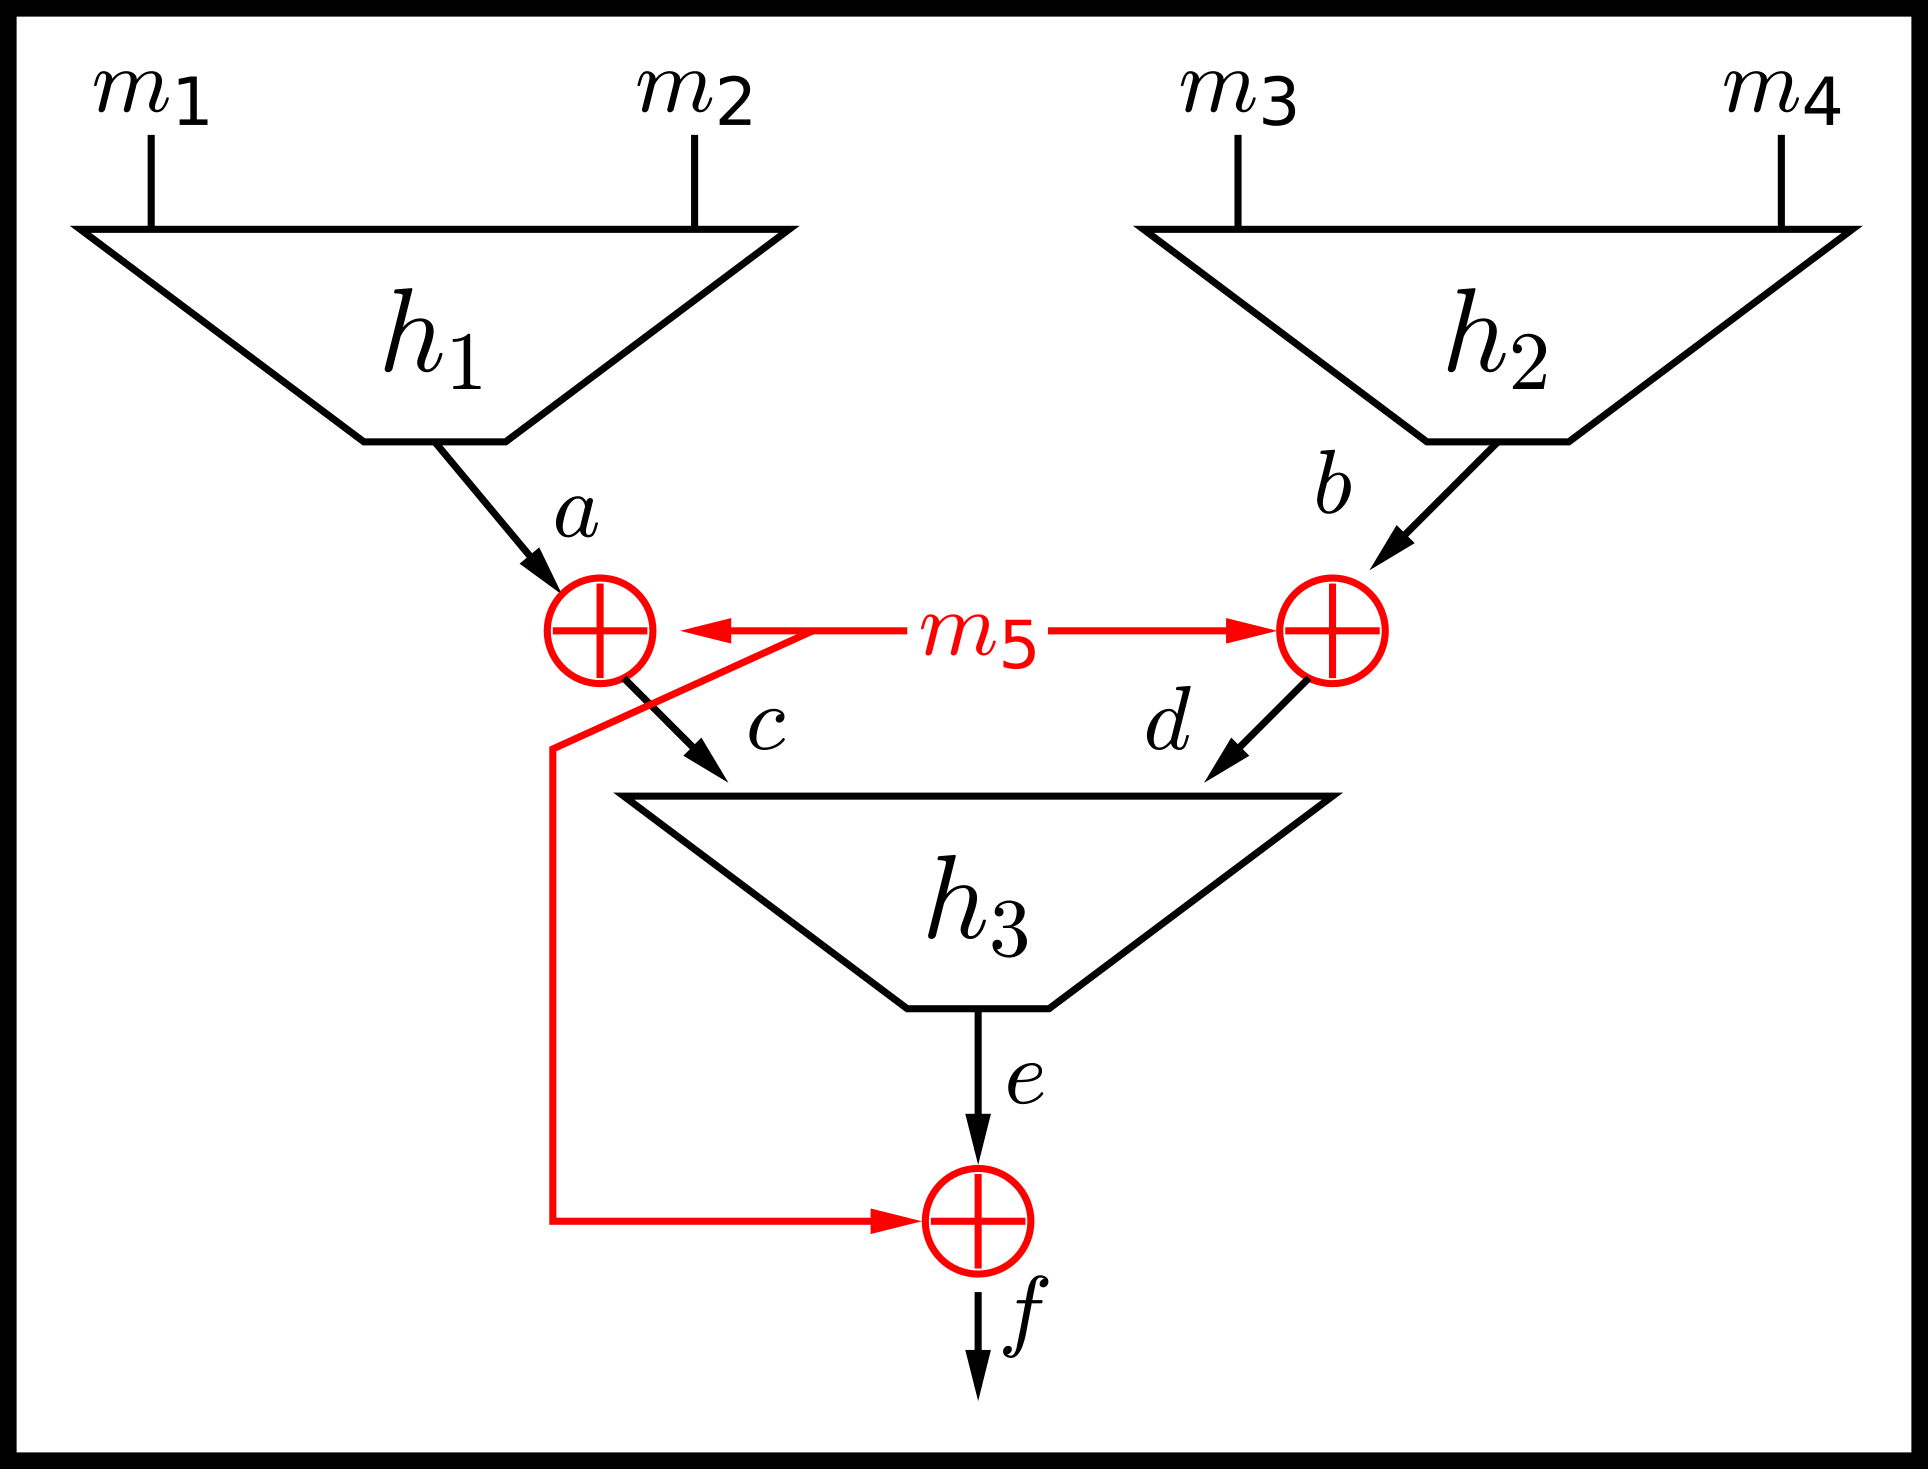
\includegraphics[]{images/Methods/abcd_paperT5_block_depiction.png}
\caption{Depiction of one $T5$ compression call with five inputs $m_1, m_2, m_3, m_4, m_5$, also denoted as one $T5$ \textit{block}.~\cite{T5_paper}} % m's are somehow cut at the top but ok
\label{img:t5_paper_block_depiction}
\end{figure}